\documentclass[10pt,a4paper]{article}

% ---------------------------------------------------------------------------
% Figures first: the seven figures of the consolidated note's section 28 and the summary figure the 25 September
% call asked for, every panel from frozen outputs. Build: cd reports && tectonic -X compile figures-first-2026-10-06.tex
% Figures: python tools/make_figures_first.py (3, 4, 7, summary); tools/make_gaussian_sanity.py (2);
% tools/make_field_sweep_figs.py (5); tools/make_field_runtime_fig.py (6); figure 1 is TikZ (figures/ff-method.tex).
% ---------------------------------------------------------------------------

\usepackage[T1]{fontenc}
\usepackage[utf8]{inputenc}
\usepackage{lmodern}
\usepackage[margin=1.9cm]{geometry}
\usepackage{microtype}
\usepackage{amsmath,amssymb}
\usepackage{booktabs}
\usepackage{graphicx}
\usepackage{float}
\usepackage{caption}
\usepackage{xcolor}
\usepackage{tikz}
\usetikzlibrary{calc,arrows.meta,positioning}
\usepackage[hidelinks]{hyperref}
\definecolor{fgblue}{HTML}{2A78D6}
\definecolor{fgink}{HTML}{52514E}
\definecolor{fgmuted}{HTML}{8A8985}
\definecolor{fgfill}{HTML}{E1E0DC}
% ===========================================================================
% Shared notation for the internal note and the compendium.
%
% Conventions follow the statistical-physics usage of the diffusion literature
% (Song et al. 2021 for the SDE formulation; Mezard-Montanari 2009 for the
% graphical-model side). Only publicly available sources are cited.
% docs/NOTATION.md is the reference for every symbol below, for the code names
% that carry them, for the collaborators' note, and for the thesis concordance.
%
% Symbol decisions that matter, fixed here once:
%
%   1. K (or K_theta) is the MARKOV TRANSITION KERNEL, everywhere and only.
%      The number of quadrature grid points is N_g. These were previously W and
%      K respectively, which collided; nothing in either document may now use
%      K for a grid size or W for a kernel. The phi^4 transfer operator
%      e^{-W} is \transfer (sans-serif T), never K.
%
%   2. The chain length is L, and every graphical-model statement is indexed by
%      sites. The ambient dimension equals it, n = L, but the two are written
%      separately because they are different concepts and the reader should not
%      have to infer the identification. The number of observed sequences is M,
%      and never the grid size.
%      A translation sentence appears at first use, because much of the
%      diffusion literature uses n for the sample count and d for the dimension.
%
%   3. The decay factor is written e^{-t} in displayed equations. Where a proof
%      abbreviates it, the abbreviation is alpha = e^{-t}, declared, never
%      alpha_t and never anything else (the code's argument `alpha` is the same
%      object).
%
%   4. Gaussian white noise eta is STANDARDISED, <eta(t)eta(t')> = delta(t-t'),
%      so the sqrt(2) is carried explicitly in both the forward and the reverse
%      SDE. This keeps Delta_t = 1 - e^{-2t} consistent throughout.
%
%   5. Vectors are bold lowercase (\vect) and matrices and tensors are bold
%      uppercase (\mat). Scalars, including single sites a_i, stay upright.
%      Anything indexed down to a scalar loses its bold.
%
%   6. BP messages are the cavity messages \lmsg_i, \rmsg_i: both EXCLUDE the
%      local likelihood ell_i, and the site marginal is \lmsg_i ell_i \rmsg_i.
%      (The collaborators' note writes alpha_i = \lmsg_i ell_i and beta_i =
%      \rmsg_i.) Posterior marginals are written out, p(a_i | x), because gamma
%      and xi are taken (6 and 7 below).
%
%   7. The chain's driving noise is eps_i with density p_eps and variance q; the
%      word "innovation" is not used (the 25 Sep call). The linear chain with
%      Laplace driving noise, not "the Laplace AR(1)".
%
%   8. Greek letters with one meaning each: gamma the phi^4 bond variance
%      (the Gaussian reference measure is \gref); xi the correlation length;
%      beta the generalised-Gaussian exponent; delta a misspecification
%      strength; h the lattice spacing (the quadrature spacing is \gridh).
% ===========================================================================

% --- Diffusion -------------------------------------------------------------
\newcommand{\Pz}{P_0}                       % clean distribution
\newcommand{\Pt}{P_t}                       % noised distribution at time t
\newcommand{\Dt}{\Delta_t}                  % 1 - e^{-2t}
\newcommand{\score}{S}                      % S(x,t) = grad log P_t(x)
\newcommand{\gwn}{\vect{\eta}}              % standardised Gaussian white noise (vector)
\newcommand{\tmin}{t_{\min}}
\newcommand{\tmax}{t_{\max}}

% Posterior mean, in bracket notation rather than E[a|x].
\newcommand{\pmean}[1]{\langle #1 \rangle_{x,t}}
\newcommand{\pmeansite}[1]{\langle a_{#1} \rangle_{x,t}}

% --- Vectors and matrices --------------------------------------------------
% Bold lowercase for vectors, bold uppercase for matrices and tensors.
\newcommand{\vect}[1]{\mathbf{#1}}
\newcommand{\mat}[1]{\mathbf{#1}}
\newcommand{\va}{\vect{a}}                  % clean chain, in R^L
\newcommand{\vx}{\vect{x}}                  % noised chain, in R^L
\newcommand{\vz}{\vect{z}}                  % standard normal draw, in R^L
\newcommand{\Sig}{\mat{\Sigma}}             % covariance
\newcommand{\Id}{\mat{I}}                   % identity

% --- Chain and graphical model --------------------------------------------
\newcommand{\nsites}{L}                     % chain length (ambient dimension n = L)
\newcommand{\nseq}{M}                       % number of observed sequences
\newcommand{\ngrid}{N_{\mathrm{g}}}         % number of quadrature grid points
\newcommand{\gridpt}[1]{u_{#1}}             % grid point
\newcommand{\gridh}{\Delta u}                % quadrature grid spacing (h is the lattice spacing)
\newcommand{\halfwidth}{A}                  % grid half-width, domain [-A, A]
\newcommand{\kernel}{K}                     % transition kernel K(a'|a)
\newcommand{\kernelth}{K_{\params}}         % parameterised transition kernel
\newcommand{\like}{\ell_t}                  % unary likelihood factor
\newcommand{\lmsg}{\overrightarrow{m}}      % forward cavity message (excludes ell_i)
\newcommand{\rmsg}{\overleftarrow{m}}       % backward cavity message (excludes ell_i)
\newcommand{\innov}{p_{\varepsilon}}          % driving-noise density
\newcommand{\corr}{\rho}                    % autoregression coefficient
\newcommand{\ivar}{q}                       % driving-noise variance
\newcommand{\ncomp}{C}                      % mixture component count

% --- The phi^4 field (docs/NOTATION.md) ------------------------------------
\newcommand{\Temp}{\Theta}                  % physical temperature (code: T)
\newcommand{\latt}{h}                       % lattice spacing
\newcommand{\bondvar}{\gamma}               % bond variance, gamma = Theta h / s^2
\newcommand{\transfer}{\mathsf{T}}          % transfer operator e^{-W}
\newcommand{\corrlen}{\xi}                  % correlation length (in sites)
\newcommand{\gref}{\mathcal{N}}             % standard Gaussian reference measure (was gamma)

% --- Estimation ------------------------------------------------------------
\newcommand{\params}{\theta}
\newcommand{\Qfun}{\mathcal{Q}}             % EM auxiliary function
\newcommand{\Xis}{\mat{\Xi}}                % expected transition statistic (a matrix)
\newcommand{\Lik}{\mathcal{L}}              % marginal log-likelihood

% --- Operators -------------------------------------------------------------
\newcommand{\E}{\mathbb{E}}
\newcommand{\Prob}{\mathbb{P}}
\newcommand{\Reals}{\mathbb{R}}
\newcommand{\Cov}{\operatorname{Cov}}
\newcommand{\Var}{\operatorname{Var}}
\newcommand{\KL}{D_{\mathrm{KL}}}
\newcommand{\normal}[2]{\mathcal{N}\!\left(#1,#2\right)}
% Gaussian moment projection, defined formally in prop-lmmse: the Gaussian with
% the same first two moments as its (normalised) argument. Named rather than
% written inline because the LMMSE proposition is a statement about WHERE this
% operator is applied, and an unnamed operator cannot carry that.
\newcommand{\Pgauss}{\Pi_{\mathrm{G}}}
\newcommand{\dd}{\,\mathrm{d}}

% --- Estimators ------------------------------------------------------------
\newcommand{\mmse}{\widehat{\va}_{\mathrm{MMSE}}}
\newcommand{\lmmse}{\widehat{\va}_{\mathrm{LMMSE}}}

% --- Pending-data guard -----------------------------------------------------
% Every number in the paper must come from the frozen batch (outputs/frozen/).
% While that batch is running, a slot that still needs a number is marked with
% \needsdata{what}, which renders in loud red with a bracket. It is deliberately
% impossible to miss in a built PDF, so a placeholder cannot be mistaken for a
% result. `tools/check_no_placeholders.sh` greps for it and fails the build if
% any survive.
\providecommand{\needsdata}[1]{{\bfseries\color{red}[PENDING: #1]}}

% --- Repository pointers (shared by the note and the compendium) ------------
% The arrow is drawn only when there IS a second component to point at.
% Four call sites pass an empty second argument to mean "the whole file", and
% those were rendering as "path/to/file.py -> produces the numbers above",
% a dangling arrow running into the prose.
\providecommand{\codepath}[1]{\texttt{\small #1}}
\providecommand{\coderef}[2]{%
  \codepath{#1}\ifx\relax#2\relax\else\,$\rightarrow$\,\texttt{\small #2}\fi}
\providecommand{\codefile}[1]{\texttt{\small #1}}

\newcommand{\code}[1]{\texttt{\small #1}}
\setlength{\parskip}{0.3em}
\graphicspath{{figures/}{../paper/figures/}}

\begin{document}

\begin{center}
{\Large\bfseries Figures first}\\[0.25em]
{\normalsize The decisive figures of the consolidated note's plan, from frozen outputs}\\[0.35em]
{\footnotesize 6 October 2026 \textperiodcentered\ branch \code{claude/phi4-field-2026-10-01} \textperiodcentered\
notation \code{docs/NOTATION.md}, metrics \code{docs/METRICS.md}}
\end{center}

\noindent The consolidated note (section 28) and the call of 25 September ask for five or six decisive figures before
the prose, and a summary figure that ``really shows everything you want to show''. This document is that selection,
for choosing: the seven figures of the note's plan, each built from frozen outputs only and named by the experiment
that produced it, and the summary. Nothing here is new data except E39 (figure 2); E40 (the FFT transition) and the
sixteen-seed replications E35x/E36x are reported in the field report.

\noindent\textbf{In one paragraph.} The estimator learns the local law of a Markov chain from noisy sequences by EM and
turns it into a score by exact inference on the chain (figure~1); on the Gaussian chain it reproduces the closed-form
score and the Kalman smoother to $2\times10^{-13}$ (figure~2). On the Laplace chain the learned mixture kernel beats the
Gaussian score wherever non-Gaussian structure survives the noise, and every network at every level (figure~3); with
128 sequences it is more accurate than the best network with 2048 (figure~4). On the $\phi^4$ field the same mixture
kernel falls onto the linear floor, because its drift is linear, while a five-parameter site energy reaches 3--17\,\%
of the floor at $M=2048$ and the networks are worse than the floor from $\Theta=0.5$ on (figure~5 and the field
report). Grid BP costs 0.5--2\,ms per sequence, 6 to 120 times a network's, for an error 14 to 32 times smaller
(figure~6), and an FFT transition does not change that at these grid sizes (E40). Under a global latent the
first-order kernel is 1.5--1.7 times worse than the linear floor, and the same kernel on the augmented state repairs
it (figure~7).

\begin{figure}[H]\centering
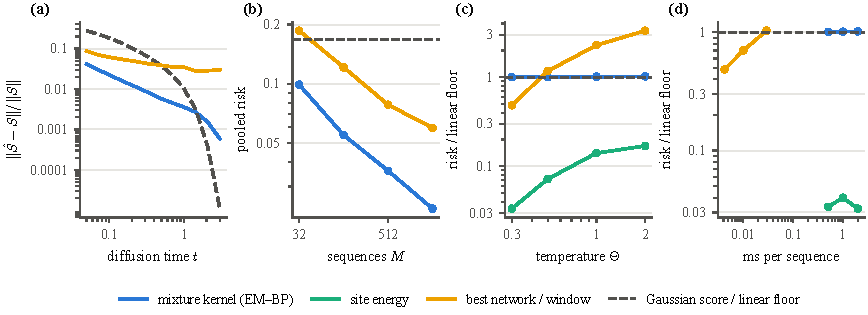
\includegraphics[width=\textwidth]{ff-summary.pdf}
\caption*{\textbf{Summary figure.} (a)~Per-level score error on the Laplace chain at $M=2048$ (E28). (b)~Pooled risk against the number of
training sequences on the Laplace chain (E02a, E03). (c)~Risk over the linear floor across temperature on the $\phi^4$
field at $M=2048$ (E33). (d)~Risk over the linear floor against inference cost on the field at $h=1$, $0.5$, $0.25$
(E33, E24x). Blue: the paper's mixture kernel (EM--BP); green: the site energy; yellow: the best network in (a, b), the
window head in (c, d); dashed: the Gaussian score or linear floor.}
\end{figure}

\section*{1. The method}
\begin{figure}[H]\centering
%% Figures-first figure 1 (the consolidated note, section 28): the method -- learn the local law, infer globally.
%% Top row: EM on noisy sequences (E-step = BP pair marginals summed into Xi; M-step = the kernel's update; the loop).
%% Bottom row: the learned kernel inside BP at any level t; Tweedie turns the posterior mean into the score, which the
%% reverse SDE uses to denoise or generate. Symbols only and one-word stage labels (docs/FIGURE_TABLE_STANDARDS.md);
%% notation docs/NOTATION.md; colours tools/figstyle.py. Needs paper/notation.tex and the fg* colours.
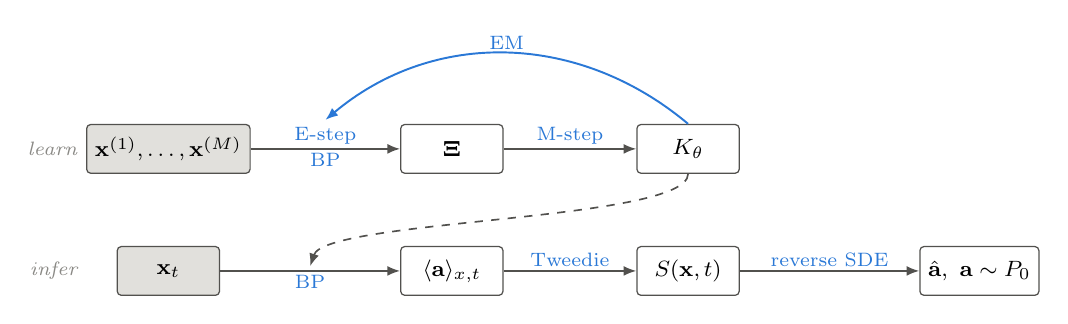
\begin{tikzpicture}[
  x=1cm, y=1cm, font=\footnotesize,
  box/.style={draw=fgink, line width=0.45pt, rounded corners=1.5pt, inner sep=3pt, minimum height=6.2mm, minimum width=13mm},
  dat/.style={box, fill=fgfill},
  stp/.style={-{Latex[length=1.6mm, width=1.25mm]}, line width=0.6pt, draw=fgink},
  emloop/.style={-{Latex[length=1.6mm, width=1.25mm]}, line width=0.7pt, draw=fgblue},
  lab/.style={text=fgblue, inner sep=1.2pt, font=\scriptsize},
  rowlab/.style={anchor=east, text=fgmuted, font=\scriptsize\itshape, inner sep=0pt},
]
  % learning row
  \node[dat] (data) at (0, 0) {$\vx^{(1)},\dots,\vx^{(\nseq)}$};
  \node[box] (xi)   at (3.6, 0) {$\Xis$};
  \node[box] (K)    at (6.6, 0) {$\kernelth$};
  \draw[stp] (data) -- node[above, lab] {E-step} node[below, lab] {BP} (xi);
  \draw[stp] (xi) -- node[above, lab] {M-step} (K);
  \draw[emloop] (K.north) to[out=140, in=40] node[above, lab] {EM} ($(data.north east)!0.5!(xi.north west)+(0,0.05)$);

  % inference row
  \node[dat] (x)  at (0, -1.55) {$\vx_t$};
  \node[box] (pm) at (3.6, -1.55) {$\pmean{\va}$};
  \node[box] (S)  at (6.6, -1.55) {$\score(\vx,t)$};
  \node[box] (gen) at (10.3, -1.55) {$\hat\va,\ \va\sim\Pz$};
  \draw[stp] (x) -- node[below, lab] {BP} (pm);
  \draw[stp] (pm) -- node[above, lab] {Tweedie} (S);
  \draw[stp] (S) -- node[above, lab] {reverse SDE} (gen);
  \draw[stp, dashed] (K.south) .. controls +(0, -0.6) and +(0.2, 0.6) .. ($(x.east)!0.5!(pm.west)+(0, 0.06)$);

  \node[rowlab] at (-1.15, 0) {learn};
  \node[rowlab] at (-1.15, -1.55) {infer};
\end{tikzpicture}

\caption{\textbf{Learn the local law, infer globally.} Top: EM on $\nseq$ noisy sequences; the E-step runs BP and
sums its pair marginals into $\Xis$, the M-step updates the kernel, and the two alternate. Bottom: the learned kernel
inside BP at any level $t$ gives the posterior mean, Tweedie's identity turns it into the score, and the reverse SDE
uses the score to denoise or generate. A direct score network learns all of the bottom row at once; here only the
kernel is learned.}
\end{figure}

\section*{2. The Gaussian sanity check}
\begin{figure}[H]\centering
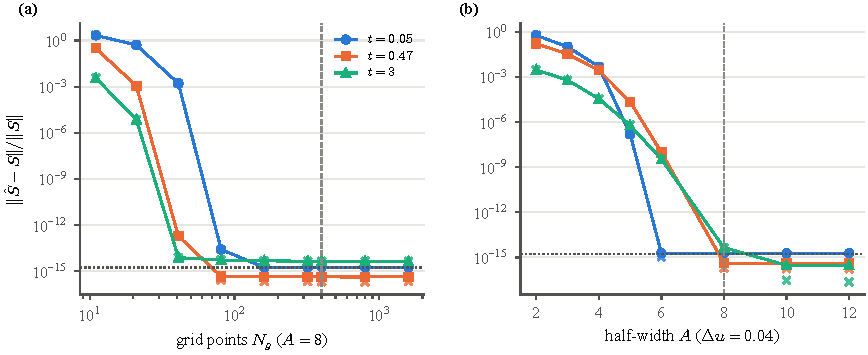
\includegraphics[width=\textwidth]{fig_gaussian_sanity.pdf}
\caption{\textbf{Grid BP converges to the closed-form score and to the Kalman smoother} (E39, Gaussian linear chain,
$\rho=0.85$, $L=32$, 256 chains, frozen). Pooled relative score error against the closed form (lines) and against an
independent Rauch--Tung--Striebel smoother (crosses), at three of the twelve levels. (a) Refining the grid at $A=8$;
(b) widening the domain at the operating spacing. Dashed: the operating grid; dotted: the smoother against the closed
form.}
\end{figure}
\noindent The smoother agrees with the closed form to $1.7\times10^{-15}$, and grid BP at $(401,8)$ with both to
$1.9\times10^{-13}$ at every level. Refining the grid converges faster than any power of the spacing and reaches
$10^{-10}$ by $N_g=81$ at the smallest levels and $41$ at the largest; at $A=3$ the truncation costs
$9.9\times10^{-2}$. The paper now states this as a proposition with its proof (appendix B). One registered clause failed
as written: moment-projected BP on the same grid is off by up to $0.26$, because the grid truncates its backward
messages, whose variance grows like $e^{2t}$; widened to $A=64$ it is exact to $10^{-15}$ up to $t=1.4$ (E39).

\section*{3. Where non-Gaussian structure pays}
\begin{figure}[H]\centering
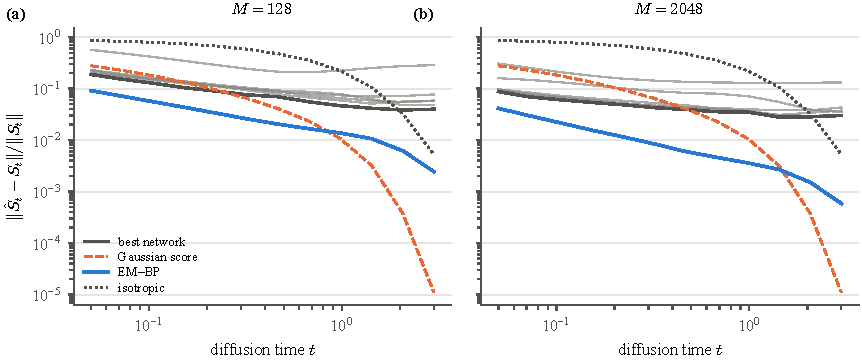
\includegraphics[width=\textwidth]{ff-nongaussian-gain.pdf}
\caption{\textbf{The gain from non-Gaussian structure, level by level} (E28, the Laplace linear chain, $\rho=0.85$,
$L=32$, sixteen seeds, frozen). Relative score error against the exact score at each level for EM--BP ($C=8$), the
Gaussian score (the LMMSE of the true covariance), the six networks of the paper (thin) and the best of them at each
level, and the isotropic prior. (a) $M=128$; (b) $M=2048$ training sequences.}
\end{figure}
\noindent EM--BP is below the best network at every level and both sizes (2 to 47\,\% of its error at $M=2048$), and
below the Gaussian score until the noise has erased the non-Gaussian structure: the two cross near $t=1$ with 128
sequences and near $t=2$ with 2048, the crossover moving with data as E28 found. At $t=0.05$ and $M=2048$ the three
errors are $0.041$ (EM--BP), $0.088$ (best network) and $0.278$ (Gaussian score).

\section*{4. Sample efficiency}
\begin{figure}[H]\centering
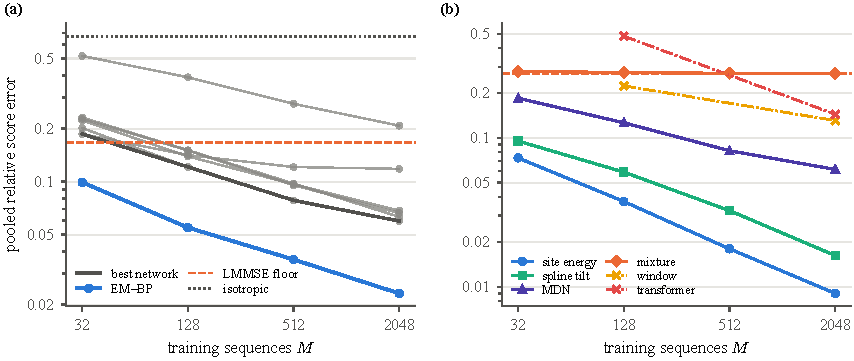
\includegraphics[width=\textwidth]{ff-sample-efficiency.pdf}
\caption{\textbf{Error against the number of training sequences.} (a) The Laplace linear chain (E03 networks, E02a
EM--BP with $C=8$; the paper's baselines table), schedule-pooled risk, sixteen seeds; dashed: the LMMSE floor;
dotted: isotropic. (b) The $\phi^4$ field at $\Theta=0.3$, $h=1$ (E33): the four kernels (risk selection) and the two
networks; dashed: the linear floor.}
\end{figure}
\noindent On the Laplace chain EM--BP is below the LMMSE floor already at $M=32$ ($0.099$ against $0.167$), where
every network is above it, and with 128 sequences ($0.055$) it beats the best network with 2048 (bidirectional GRU,
$0.060$). On the field the site energy falls from $0.073$ to $0.009$ between $M=32$ and $2048$ and the spline from
$0.095$ to $0.016$, while the mixture kernel stays on the floor ($0.27$) at every size; the networks, trained at
$M=128$ and $2048$, reach $0.13$ (window) and $0.14$ (transformer).

\section*{5. The temperature sweep}
\begin{figure}[H]\centering
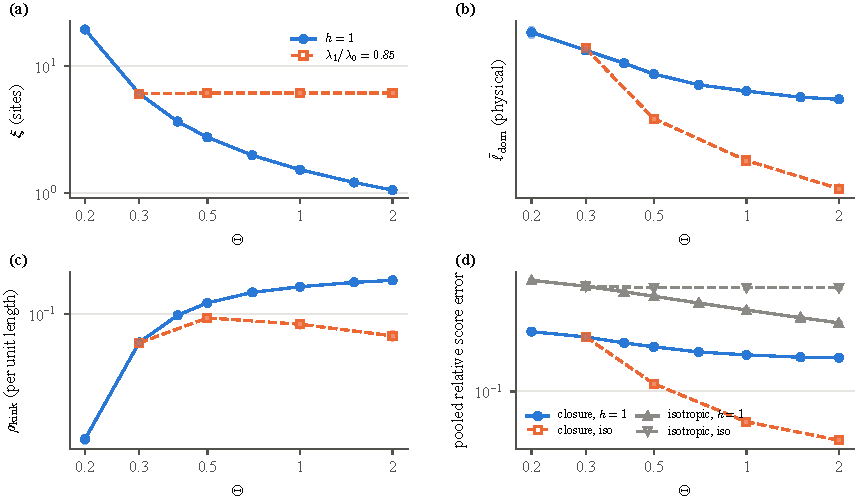
\includegraphics[width=\textwidth]{fig-field-sweep.pdf}
\caption{\textbf{The $\phi^4$ field across temperature} (E32 fixed-spacing and iso-correlation sweeps, E34; the
field report's figure). Correlation length, domain length, kink density and the score error of the linear closure
across $\Theta$.}
\end{figure}
\noindent At fixed spacing ($h=1$) the linear floor falls only from $0.30$ to $0.18$ over $\Theta=0.2$--$2$ while
kinks multiply ($0.016$ to $0.166$ per bond) and domains shorten ($9.0$ to $5.3$ sites); along the iso-correlation
line it falls from $0.269$ to $0.041$ (E32, frozen). The learned arms across $\Theta$ are panel (c) of the summary.
In one dimension there is no phase transition at $\Theta>0$; the low-temperature end is a sharp crossover.

\section*{6. Refinement and runtime}
\begin{figure}[H]\centering
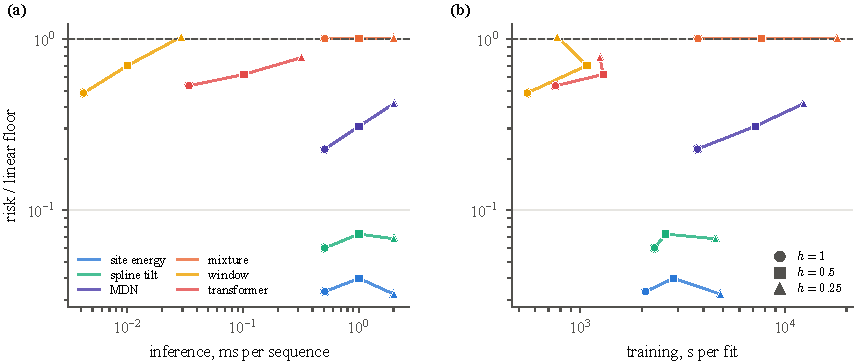
\includegraphics[width=0.92\textwidth]{fig-field-runtime.pdf}
\caption{\textbf{Accuracy against cost across the lattice spacing} (E33 risk at $M=2048$ over its linear floor,
sixteen seeds; inference from E24's exclusive-node sweep, 8 BLAS threads; training wall clock from E33, shared nodes).
Markers: $h=1$, $0.5$, $0.25$ ($L=32$, $64$, $128$). (a) Inference, ms per sequence; (b) training, s per fit.}
\end{figure}
\noindent Grid BP costs $0.5$, $1.0$ and $2.0$\,ms per sequence at $L=32$, $64$, $128$; the networks are 6 to 120
times cheaper but sit at 48--103\,\% of the linear floor, against 3--4\,\% for the site energy and 6--7\,\% for the
spline. A network trains in 9--22 minutes, an EM fit in 35 minutes to 5 hours (shared nodes). The FFT transition the
note proposes (section 9.2; E40) is accurate to second order ($6.7\times10^{-4}$ from dense BP at $N_g=401$) and
$5.8$ times slower than the dense one there on one core; tuned, it breaks even only near $N_g=3200$.

\section*{7. Misspecification and its repair}
\begin{figure}[H]\centering
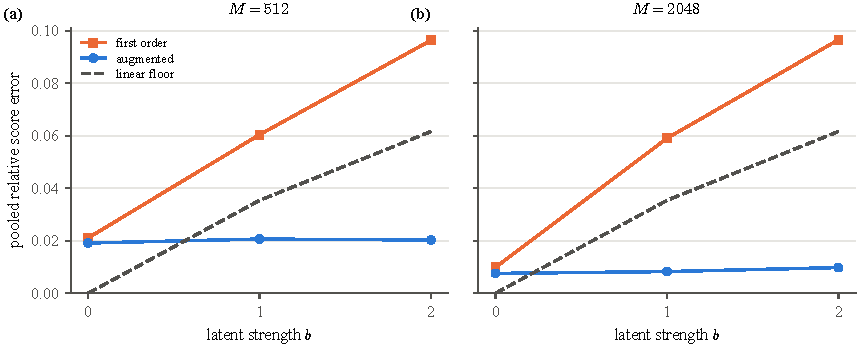
\includegraphics[width=0.86\textwidth]{ff-misspec-repair.pdf}
\caption{\textbf{A global latent the first-order kernel cannot see, and the repair by state augmentation} (E35:
$X_i=Gb+U_i$, $G=\pm1$ per sequence, $U$ the Gaussian linear chain at $\rho=0.85$; closed-form exact score; two
seeds, frozen). The mixture kernel on $X$ (first order) and the same kernel on the state $(X_i,G)$ tied by
reflection (augmented), against the linear floor, over the latent strength $b$. (a) $M=512$;
(b) $M=2048$.}
\end{figure}
\noindent At $b=0$ the arms agree and the floor is the exact score (the chain is Gaussian). With the latent the
first-order kernel's risk grows with $b$ and does not fall when $M$ quadruples: it is 1.5 to 1.7 times worse than the
linear floor at $b=1$ and $2$. The augmented kernel, with the same parameter count, stays flat; at $b=2$, $M=2048$ its
risk is $8.6$ and $17.9$ times smaller than the first-order one in the two seeds. Sixteen seeds (E35x) are queued on
the cluster, and the figure will be redrawn from them.

\end{document}
